\title{Biltré}
\author{Bergur Snorrason}
\date{\today}

\begin{document}

\frame{\titlepage}

\env{frame}
{
	\frametitle{Dæmi}
	\env{itemize}
	{
		\item<1-> Gefinn er listi með $n$ tölum.
		\item<2-> Næst koma $q$ fyrirspurnir, þar sem hver er af einni af tveimur gerðum:
		\env{itemize}
		{
			\item<3-> Bættu $k$ við $i$-tu töluna.
			\item<4-> Reiknaðu summu allra talna á bilinu $[i, j]$.
		}
		\item<5-> Einföld útfærlsa á þessum fyrirspurnum gefur okkur
					$\mathcal{O}($\onslide<6->{$\,1\,$}$)$ fyrir þá fyrri og
					$\mathcal{O}($\onslide<7->{$\,n\,$}$)$ fyrir þá seinni.
		\item<8-> Þar sem allar (eða langflestar) fyrirspurnir gætu verið af seinni gerðin yrði lausnin í heildin 
					$\mathcal{O}($\onslide<9->{$qn$}$)$.
		\item<10-> Það er þó hægt að leysa þetta dæmi hraðar.
		\item<11-> Algengt er að nota til þess \emph{biltré} (e. \emph{segment tree}).
	}
}

\env{frame}
{
	\frametitle{Biltré}
	\env{itemize}
	{
		\item<1-> Biltré er tvíundartré sem geymir svör við vissum fyrirspurnum af seinni gerðinni.
		\item<2-> Rótin geymir svar við fyrirspurninni \texttt{1 n} 
					og ef nóða geymir svarið við \texttt{i j} þá geyma börn hennar svör við \texttt{i m}
					og \texttt{(m + 1) j}, þar sem $m$ er miðja heiltölubilsins $[i, j]$.
		\item<3-> Þær nóður sem geyma svar við fyrirspurnum af gerðinni \texttt{i i} eru lauf trésins.
		\item<4-> Takið eftir að laufin geyma þá gildin í listanum og aðrar nóður geyma summu barna sinna.
		\item<5-> Þegar við útfærum tréð geymum við það eins og hrúgu.
	}
}

\env{frame}
{
	\frametitle{Mynd af biltré, $n = 4$}
	\env{figure}
	{
		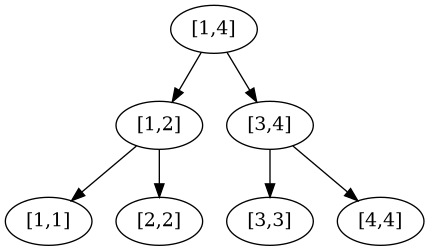
\includegraphics[scale=0.5]{fig/mynd2.png}
	}
}

\env{frame}
{
	\frametitle{Mynd af biltré, $n = 7$}
	\env{figure}
	{
		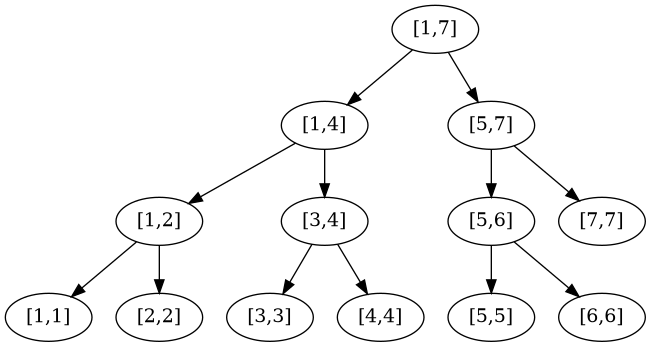
\includegraphics[scale=0.3]{fig/mynd3.png}
	}
}

\env{frame}
{
	\env{itemize}
	{
		\item<1-> Gerum ráð fyrir að við höfum biltré eins og lýst er að ofan og látum $H$ tákna hæð trésins.
		\item<2-> Hvernig getum við leyst fyrirspurnirnar á glærunni á undan, og hver er tímaflækjan?
		\item<3-> Fyrri fyrirspurnin er einföld.
		\item<4-> Ef við eigum að bæta $k$ við $i$-ta stakið finnum við fyrst laufið sem svarar til fyrirspurnar \texttt{i i},
					bætum $k$ við gildið þar og förum svo upp í rót í gegnum foreldrin og uppfærum á leiðinni gildin í þeim nóðu sem við lendum í.
		\item<5-> Þar sem við heimsækjum bara þær nóður sem eru á veginum frá rót til laufs (mest $H$ nóður)
					er tímaflækjan á fyrri fyrirspurninni $\mathcal{O}($\onslide<6->{$\,H\,$}$)$.
	}
}

\env{frame}
{
	\selectcode{code/daemi1-segmenttree.c}{24}{38}
}

\env{frame}
{
	\env{itemize}
	{
		\item<1-> Seinni fyrirspurnin er ögn flóknari.
		\item<2-> Auðveldast er að ímynda sér að við förum niður tréð og leitum að hvorum endapunktinum fyrir sig.
		\item<3-> Á leiðinni upp getum við svo pússlað saman svarinu, eftir því hvort við erum að skoða hægri eða vinstri endapunktinn.
		\item<4-> Til dæmis, ef við erum að leita að hægri endapunkti $x$ og komum upp í bil $[i, j]$ þá bætum við gildinu í nóðu
			$[i, m]$ við það sem við höfum reiknað hingað til ef $x \in [m + 1, j]$, en annars bætum við engu við (því $x$ er hægri endapunkturinn).
		\item<5-> Við göngum svona upp þar til við lendum í bili sem inniheldur hinn endapunktinn.
		\item<6-> Með sömu rökum og áðan er tímaflækjan $\mathcal{O}($\onslide<7->{$\,H\,$}$)$.
	}
}

\env{frame}
{
	\env{figure}
	{
		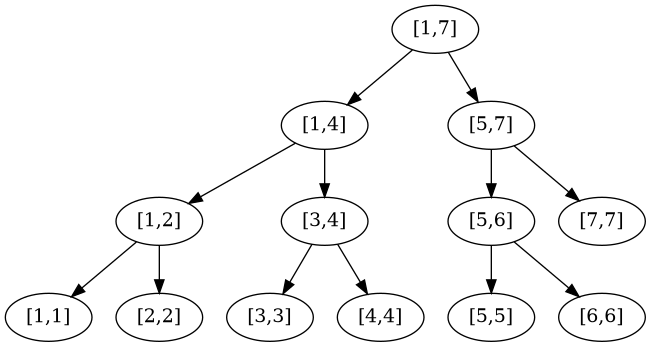
\includegraphics[scale=0.3]{fig/mynd3.png}
		\env{itemize}
		{
			\item<1-> Látum $f(i, j)$ tákna svar við fyrirspurninni \texttt{i j} og skoðum nokkur dæmi.
			\env{itemize}
			{
				\item<2-> $f(1, 3) = f(1, 2) + f(3, 3)$.
				\item<3-> $f(2, 5) = f(2, 2) + f(3, 4) + f(5, 5)$.
				\item<4-> $f(1, 6) = f(1, 4) + f(5, 6)$.
				\item<5-> $f(3, 6) = f(3, 4) + f(5, 6)$.
			}
		}
	}
}

\env{frame}
{
	\frametitle{Biltré í \texttt{C}}
	\selectcode{code/daemi1-segmenttree.c}{10}{22}
}

\env{frame}
{
	\frametitle{Tímaflækja biltrjáa}
	\env{itemize}
	{
		\item<1-> Þar sem lengd hvers bils sem nóða svarar til helmingast þegar farið er niður tréð er
					$\mathcal{O}(H) = \mathcal{O}($\onslide<2->{$\log n$}$)$.
		\item<3-> Við erum því komin með lausn á upprunalega dæminu sem er $\mathcal{O}($\onslide<4->{$q \cdot \log n$}$)$.
		\item<5-> Þetta væri nógu hratt ef, til dæmis, $n = q = 10^6$.
		\item<6-> Tökum annað dæmi.
	}
}

\env{frame}
{
	\frametitle{Annað dæmi}
	\env{itemize}
	{
		\item<1-> Fyrsta lína inntaksins inniheldur tvær jákvæðar heiltölur, $n$ og $m$, minni en $10^5$.
		\item<2-> Næsta lína inniheldur $n$ heiltölur, á milli $-10^9$ og $10^9$.
		\item<3-> Næstu $m$ línur innihalda fyrirspurnir, af tveimur gerðum. 
		\item<4-> Fyrri gerðin hefst á \texttt{1} og inniheldur svo tvær tölur, $x$ og $y$. Hér á að setja $x$-tu töluna sem $y$.
		\item<5-> Seinni gerðin hefst á \texttt{2} og inniheldur svo tvær tölu,
			$x$ og $y$. Hér á að prenta út stærstu töluna á hlutbilinu $[x, y]$ í talnalistanum.
		\item<6-> Hvernig leysum við þetta?
	}
}

\env{frame}
{
	\env{itemize}
	{
		\item<1-> Við getum leyst þetta með biltrjám.
		\item<2-> Í stað þess að láta nóður (sem eru ekki lauf) geyma summu barna sinna, þá geyma þær stærra stak barna sinna.
	}
}

\env{frame}
{
	\frametitle{Lausn}
	\selectcode{code/daemi2-segmenttree.c}{11}{40}
}

\env{frame}
{
	\env{itemize}
	{
		\item<1-> Leysa má ýmis dæmi af þessari gerð, með biltrjám.
		\item<2-> Þessi dæmi eru yfirleitt kölluð \emph{punkt-uppfærlsur, bil-fyrirspurnir} (e. \emph{point-update, range-query}).
		\item<3-> Algengt er að sýna næst hvernig nota megi biltré til að leysa \emph{bil-uppfærslur, punkt-fyrirspurnir}
					(e. \emph{range-update, point-query}).
		\item<4-> Þetta er, í grófum dráttum, gert með því að snúa trjánum við.
		\item<5-> Við munum ekki skoða þetta.
		\item<6-> Við tökum frekar fyrir \emph{lygn biltré}.
		\item<7-> Þau leyfa okkur að leysa \emph{bil-uppfærlsur, bil-fyrirspurnir} (e. \emph{range-update, range-query}).
	}
}

\env{frame}
{
	\frametitle{Lygn dreifing}
	\env{itemize}
	{
		\item<1-> Sem beinagrind munum við nota biltrjáa útfærsluna sem við notuðum til að leysa fyrsta dæmið.
		\item<2-> Við munum nú láta fyrri fyrirspurnina, \texttt{i j k}, þýða ``Bættu $k$ við allar tölur á bilinu $[i, j]$''.
		\item<3-> Uppfærslan er framkvæmd á svipaðan hátt og fyrirspurnirnar eru.
		\item<4-> Við geymum í öðrum tréi þær uppfærslur sem við eigum eftir að framkvæma.
		\item<5-> Í hverri endurkvæmni (bæði uppfærlum og fyrirspurnum) dreifum við uppfærslunum í nóðunni niður á við.
		\item<6-> Þetta kallast \emph{lygn drefing} (e. \emph{lazy propagation}), því við framkvæmum hana bara þegar nauðsyn krefur.
		\item<7-> Ef biltré hefur lygna dreifingu köllum við það \emph{lygnt biltré} (e. \emph{segment tree with lazy propagation}).
	}
}

\env{frame}
{
	\env{itemize}
	{
		\item<1-> Látum $i < j$ vera heiltölur þannig að bilið $[i, j]$ svara til nóðu í biltréi og $m$ vera miðpunkt heiltölu bilsins $[i, j]$.
		\item<2-> Gerum ráð fyrir að við eigum eftir að framkvæma uppfærslu \texttt{i j k}.
		\item<3-> Næst þegar við köllum á \texttt{query\_rec(i, j, ...)} eða \texttt{update\_rec(i, j, ...)}
					þá munum við dreifa uppfærslunni \texttt{i j k}.
		\item<4-> Eftir dreifinguna munum við ekki eiga eftir uppfærslu á bilinu $[i, j]$, en við munum eiga eftir uppfærslurnar
					\texttt{i m k} og \texttt{(m + 1) j k}.
		\item<5-> Þegar við dreifum uppfærslunni \texttt{i i k} þá nægir að uppfæra tilheyrandi lauf í biltrénu.
	}
}

\env{frame}
{
	\env{itemize}
	{
		\item<1-> Áðan var sagt ``laufin geyma þá gildin í listanum og aðrar nóður geyma summu barna sinna''.
		\item<2-> Þetta gildir ekki fyrir lygn biltré.
		\item<3-> Nóður lygna biltrjáa þurfa að geyma summu barna sinna,
					ásamt því að geyma þá summu sem fengist eftir allar óframkvæmdar uppfærslur afkomenda hennar.
		\item<4-> Þegar við ferðumst í gegnum tréð til að finna hvert við eigum að setja uppfærsluna uppfærum við tréð jafn óðum.
		\item<5-> Til dæmis, ef við viljum framkvæma uppfærsluna \texttt{i j k} þá þurfum við að bæta $k \cdot (j - i + 1)$ við rót biltrésins,
					því rótin geymir summu allra stakana.
	}
}

\env{frame}
{
	\selectcode{code/segmenttree-le.c}{10}{44}
}

\env{frame}
{
	\env{itemize}
	{
		\item<1-> Nú hefur \texttt{query(...)} sömu tímaflækju og í hefðbundnum biltrjám, það er að segja $\mathcal{O}($\onslide<2->{$\log n$}$)$.
		\item<3-> Loks fæst (með sömu rökum og gefa tímaflækju \texttt{query(...)}) að \texttt{update(...)} er
					$\mathcal{O}($\onslide<4->{$\log n$}$)$.
	}
}

\env{frame}
{
}

\end{document}
